\chapter{Background}
\section{Communicating Sequential Processes} \label{csp_section}
Communicating Sequential Processes (CSP) was discovered by Tony Hoare, it provides us with a mathematical notation for defining processes and interactive systems \cite{csp_paper}. CSP provides a framework for reasoning about the behaviour of concurrent systems which has influenced distributed algorithms \cite{distributed_algorithms_na_lynch}, model checking \cite{model_checking} and many other related research fields. This section will give a brief introduction to some process algebra introduced to model some simple parallel processes.
\par
CSP defines processes and events. The alphabet of a process, $\alpha P$ is the set of all events. For example, the alphabet of a student process $S$ could consist of two events.
\[
\alpha S = \{study, sleep\}
\]
The process with the alphabet $A$ which never engages in the events of A is called $STOP_A$. We can now construct a sequence of events for a process.
\[
(study \rightarrow (sleep \rightarrow (study \rightarrow STOP_{\alpha S})))
\]
Using the same alphabet, we now define two simple processes modeling a student $S$ and a strict teacher $T$, who never accepts students sleeping.
\[
\begin{aligned}
& L = (study \rightarrow sleep \rightarrow L) \\
& T = (study \rightarrow study \rightarrow T) 
\end{aligned}
\]
Note that both processes are recursively defined, hence a valid \texttt{trace} for $L$ could be $\langle study, sleep, study, sleep \rangle$.
\par
We can now introduce the process algebra for concurrency, using the parallel composition operator (`||'). To help reason about concurrent processes, we also introduce $\mu X \bullet F(X)$ to define recursive processes. This now lets us denote a process that behaves like a system of composed processes, where both processes have the same algebra $\alpha S$.
\[
(T \,||\, L)    
\]
Using the definitions for $T$ and $L$, and the recursive process definition, we have.
\[
(T \,||\, L) = (study \rightarrow STOP)    
\]
This is the composition of both processes. As both begin with a \texttt{study} event, so does the composition. However, after \texttt{study} each component process is prepared to take another event but as these are different, the processes can not agree on what event to take next. The resulting \texttt{STOP} is known as a deadlock. Alternatively, had the student and teacher processes been defined with behaviour that composes without deadlock, we could describe that behaviour with process algebra.
\[
\begin{aligned}
& L = (study \rightarrow L \,|\, sleep \rightarrow L) \\
& T = (study \rightarrow study \rightarrow T) \\
& \\ 
& (T \,||\, L) = \mu X \bullet (study \rightarrow study \rightarrow X)
\end{aligned}
\]
Note how now under the composed behaviour, the sleep event never occurs. The composition can be described as a single process. Also, note the use of recursion with the fixed-point operator $\mu X \bullet F(X)$ \cite[p.74]{csp_paper}, where $X$ marks recursion under the composed process.
\par
Finally, we will briefly look at how Hoare modelled communication between processes. Hoare designed communication over channels. A pair $c.v$ represents communication taking place over a channel $c$ and $v$ is the value of a message being passed. Hoare describes the set of all messages that a process $P$ can communicate on channel $c$ as $\{ v \,|\, c.v \in \alpha P \}.$
\[
\alpha c(P) = \{ v \,|\, c.v \in \alpha P \}
\]
Functions to extract the channel and message components from the pair $c.v$ are also defined.
\[
\begin{aligned}
& channel(c.v) = c \\
& message(c.v) = v
\end{aligned}
\]
With this understanding, we can finally model sending and receiving messages to channels. Given a process $P$ and a value $v \in \alpha c(P)$, a process can output $v$ on the channel $c$.
\[
(c!v \rightarrow P)
\]
Similarly, we can read messages from channels. A process can input any value $x$ on the channel $c$, and then behave under $P(x)$.
\[
(c?x \rightarrow P(x))
\]
That concludes a brief overview of the process algebra proposed by Tony Hoare. We saw how event sequencing constructs processes, how processes can be composed and the special communication event $c.v$ which allows message-passing over channels. Tools have been built from similar syntax and concepts, for example, Promela \ref{sec:promela}, which models channels and messages with a similar approach.
\section{Model Checking}
Model checking is the process of determining if a finite-state machine (FSM) is correct under a provided specification. It typically involves enumerating all possible states of an FSM and ensuring the correctness of each state. For example, given a model M and a property $\varphi$, if no state of M violates $\varphi$, then we can say M satisfies $\varphi$. In software development, model checkers are beneficial in providing guarantees for safety-critical systems as well as concurrent systems. Concurrent systems can often cause issues with uncommon instruction execution interleavings that are not easily identifiable until long into a runtime. For example, deadlocks can occur when instructions being run by two processes are dependent on one another making progress. A simple example of a deadlock that can occur is the following interleaving of instructions executed by two processes, $\tau_1$ and $\tau_2$. 
\[
\begin{aligned}
& \tau_1: \text{ acquire lock A} \\
& \tau_2: \text{ acquire lock B} \\
& \tau_1: \text{ acquire lock B} \\
& \tau_2: \text{ acquire lock A}
\end{aligned}
\]
This simple interleaving results in $\tau_1$ blocking until it can acquire lock B, and $\tau_2$ blocking until it can acquire lock A, hence the program is in a deadlock. Due to the nature of concurrent systems, we could run our program and never experience this interleaving of instructions from occurring, hence we could deem our program deadlock-free. By instead abstracting our program as a model, and verifying the correctness using a model checker, we could exhaustively check all possible states (interleavings of concurrent processes) and catch this deadlock. 
\par
Alongside determining progress can be made within a system, model checkers are also used to guarantee the correctness of a specification. To demonstrate, we model a very simple 24-hour clock, where at each time step, we progress time by an hour.
\[
\begin{aligned}
& \tau_1: \text{time} \leftarrow \text{time} + 1
\end{aligned}
\]
Unlike the previous example, this process can always make progress so will not result in a deadlock, however, it is not a correct implementation of a 24-hour clock. We would like our 24-hour clock to only represent times in the range 1 to 24. By introducing a specification alongside our model, we can use a model checker to determine if all the states of our program adhere to the specification. In this instance, we would just need to specify a bound over our time variable.
\[
\{ \text{time} \mid \text{time} \in \mathbb{N}, 1 \leq \text{time} \leq 24 \}
\]
This is a simple example of a specification, that we can write in a specification language and use in tandem with our model to check the correctness of using a model checker.
\subsection{A Comparison Of Model Checkers}
Many model checkers have been invented for this reason, each with different focuses and specification languages. This section will comment on some of the more common model checkers and discuss their functionalities. \\
\subsubsection*{\textbf{PAT}}
Process Analysis Toolkit (PAT) is a self-contained framework to support composing, simulating and reasoning of concurrent, real-time systems \cite{pat}. PAT is based on Tony Hoare's CSP and extends the language using its library called CSP\#. CSP\# is a superset language of the original CSP, hence all classical CSP models can be verified with PAT. PAT has shown to be capable of verifying classical concurrent algorithms such as the dining philosophers problem. Alongside its verification capabilities, the PAT toolkit can be used to simulate real-world scenarios over specifications. 
\par
PAT's ability to determine the correctness of classical process algebra means it is a strong, widely applicable model checker.

\subsubsection*{\textbf{BLAST}}
BLAST is an automatic verification tool for checking the temporal safety properties of C programs. Given a C program and a temporal safety property, BLAST either statically proves the program satisfies the property or provides an execution path that exhibits a violation of the property \cite{blast}.
\par
Where BLAST is more interesting than PAT is that it no longer relies on process algebra. The model checker is capable of being run directly on a subset of C programs, no intermediate modelling is required. As an end-user tool, this is more generally applicable than PAT, there is no burden on developers to think about how to model their systems with process algebra and instead can directly get safety guarantees from their programs. BLAST handles the translation of C programs to an abstract reachability tree (ART), a labeled tree that represents a portion of the reachable state space of the program. Using a context-free reachability algorithm on this representation of a C program means temporal properties can be checked without the end programmer being required to think about what the control-flow automata for the program will look like.
\par
BLAST falls short when model-checking large C programs. More importantly, it is unable to provide any guarantees on concurrent programs. A strong driving factor in why developers choose to design systems in Elixir is its concurrent capabilities. 

\subsubsection*{\textbf{PRISM}}
PRISM is a probabilistic model checker, a tool for formal modelling and analysis of systems that exhibit random behavior or probabilistic behavior \cite{prism}. It has been used to analyse systems implementing random distributed algorithms.

\subsubsection*{\textbf{TLC}}
In 1980, Leslie Lamport discovered the Temporal Logic of Action (TLA) \cite{tla}. TLA is a logic system for specifying and reasoning about concurrent systems. Both the systems and their properties are represented in the same logic so that the assertion that a system meets its specification can be expressed by a logical implication.
\par
TLA is capable of specifying complex systems but in a typically verbose manner. Leslie Lamport introduced TLA+ \cite{tlaplus}, combining mathematical ideas with concepts from programming languages to create a specification language that would allow mathematicians to write specifications in 20 lines as opposed to 20 pages.
\begin{figure}[H]
    \begin{verbatim}
    ---------------------- MODULE HourClock ----------------------
    EXTENDS Naturals
    VARIABLE hr
    HCini == hr \in (1 .. 12)
    HCnxt == hr' = IF hr # 12 THEN hr + 1 ELSE 1
    HC == HCini /\ [][HCnxt]_hr
    --------------------------------------------------------------
    THEOREM HC => []HCini
    ==============================================================
    \end{verbatim}
    \caption{An example TLA+ Specification for an HourClock \cite{tlaplus}}
    \label{fig:hourclock_spec}
\end{figure}
\par
Furthering on from Leslie Lamport's discovery of these specification languages, Lamport created TLC \cite{tlc}, a model checker for the verification of TLA+ specifications. Similarly to BLAST, TLC builds a finite-state machine from the specification so the model checker can verify and debug invariance properties over it. TLC has been used to verify many large-scale, real-world systems specified in TLA+. Not only does it verify temporal properties of TLA+ specifications, but it can also model check PlusCal \cite{pluscal} algorithms. PlusCal is an algorithm language aimed to resemble that of pseudocode, but PlusCal algorithms can be automatically translated to TLA+ specifications to be reasoned about formally with TLC. We have already come across the concept of model-checking algorithms as opposed to specifications with BLAST, but instead of being strictly bound to the C programming language, PlusCal provides a more general framework agnostic of a choice of programming language allowing developers to separate reasoning about algorithms from their respective programs.

\subsubsection*{\textbf{SPIN}}
SPIN is an efficient verification system for models of distributed software systems. It has been used to detect design errors in applications ranging from high-level descriptions of distributed algorithms to detailed code \cite{spin}. Spin has a specification language, Process Meta Language (Promela), which the model checker uses to prove the correctness of asynchronous process interactions. Spin supports asynchronous process communication through channels, where processes can send and receive messages. Spin constructs labeled transition systems for respective processes from Promela specifications which it goes on to use for scheduling and to reason about properties of the model. Because many programming languages, such as GO \cite{go} rely on the creation of channels for asynchronous communication between processes, Promela becomes a natural solution to modelling these systems.
\begin{lstlisting}[caption={Example of a Promela specification that enqueues a message in a channel}]
mtype = { HELLO };
chan channel = [10] of { mtype };

init {
    channel ! HELLO;
}
\end{lstlisting}

\section{Theorem Proving}
Theorem proving is another process to verify programs. In theorem proving, axioms are applied to a set of statements to determine if a particular statement holds. For example, Z3 \cite{z3} is a satisfiability modulo theories (SMT) solver developed by Microsoft that can verify propositional logic assertions.
\subsection{Hoare Logic}
Hoare Logic was discovered in 1969 by Tony Hoare \cite{hoare_logic}. Hoare Logic defines the Hoare Triple, an essential idea in describing how code execution changes the state of a computation. A Hoare Triple is composed of a pre-condition assertion $P$, a post-condition assertion $Q$, and a command $C$.
\[
\{P\}C\{Q\}
\]
Note how the postcondition is the same as the precondition for this command.
\par
Hoare Logic provides axioms and inference rules required to construct a simple imperative programming language. If $P$ holds in the given state and $C$ terminates, then $Q$ will hold after. Below is an example of a simple Hoare Triple for the \texttt{skip} command, which leaves the program state unchanged.
\[
\overline{\{P\}\text{skip}\{P\}}
\]
Hoare describes many more rules that allow for assignment, composition, consequence and so forth. These rules have led to the development of modern-day theorem provers, such as Z3, which will detailed more later.
\section{Elixir TODO = discuss array argument reductions, qualified calls}
Elixir is a dynamic, functional language for building scalable and maintainable applications \cite{elixir}. Elixir programs run on the BEAM virtual machine\cite{beam}, which is also used to implement the Erlang programming language \cite{erlang}. Elixir was designed by José Valim and first released in 2012. Elixir is built on top of Erlang and hence inherits many of the abstractions designed for building distributed systems.
\par
BEAM is a virtual machine that executes user programs in the Erlang Runtime System (ERTS). BEAM is a register machine where all instructions operate on named registers containing Erlang terms such as integers or tuples.
\par
Elixir has begun to see use in industry, in particular in domains such as telecoms and instant messaging. The Phoenix Framework \cite{phoenix} is a framework for building interactive web applications natively in Elixir that can take advantage of Elixir's multi-processing and fault tolerance to build scalable web applications. The audio and video communication application Discord \cite{discord} uses Elixir to manage its 11 million concurrent users and the Financial Times \cite{ft} have begun migrating from Java to Elixir to enjoy the much smaller memory usage by comparison.
\par
Elixir supports multi-processing in two key ways: nodes and processes. Each node is an instance of BEAM (a single operating system process), when an Elixir program is executed, a new instance of BEAM is instantiated for it to run on. In contrast, an Elixir process is not an operating system process. An Elixir process is lightweight in terms of memory and CPU usage (even in comparison to threads that many other programming languages favour). Elixir processes can run concurrently with one another and are completely isolated from one another. Elixir processes communicate via message passing.
\begin{lstlisting}[language=Elixir, xleftmargin=.2\linewidth, caption={An example of spawn/1 and spawn/4 in Elixir for spawning a new lightweight process and a new Elixir node}]
    # Spawn a new process
    spawn(fn -> 1 + 2 end)

    # Create a new BEAM instance
    Node.spawn(:"node1@localhost", MyModule, :start, [])
\end{lstlisting}
\subsection{Shared Memory and Message Passing}
Two key concepts in inter-process communication (IPC) are shared memory models and message passing models. They are two techniques used to allow processes to send signals or share data between each other. In a shared memory model, a shared memory region is established in which multiple processes can read and write. Figure \ref{fig:shared_memory} shows a basic example of two processes that write to a shared in-memory array. Due to how often we see shared memory used in large-scale distributed systems, much work has been done in the verification of these systems using shared memory models. For example, Jon Mediero Iturrioz used Dafny \cite{dafny} to prove the correctness of concurrent programs that implement shared memory \cite{shared_memory_verification}. 
\begin{figure}[h]
    \centering
    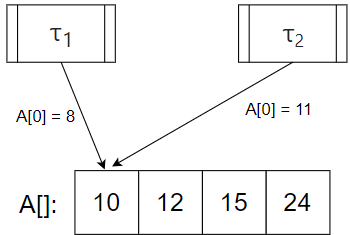
\includegraphics[width=0.4\textwidth]{images/shared_memory.png}
    \caption{An example of two processes writing to a shared in-memory array}
    \label{fig:shared_memory}
\end{figure}
\par
Elixir instead uses a message-passing model for IPC. More specifically, Elixir uses an actor-based model, where each process (actor) has its state and a message box to receive messages from other actors. Actors are responsible for sending a finite number of messages to other actors, spawning new actors and changing their behaviour based on the handling of messages received in the mailbox. Figure \ref{fig:actor_model} shows an example of how actors behave. The mailbox is not necessarily first in, first out (FIFO) but often implementations tend to be.
\begin{figure}[H]
    \centering
    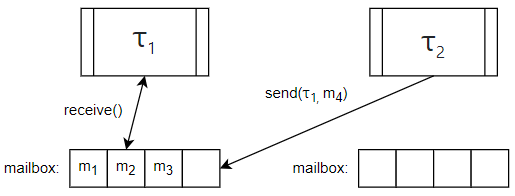
\includegraphics[width=0.6\textwidth]{images/actor_model.png}
    \caption{An example of actors sending and receiving messages under the actor model}
    \label{fig:actor_model}
\end{figure}
\par
In Elixir, a receive statement is used to read messages in the mailbox. The receive block looks through the mailbox for a message that matches a given pattern, if no messages match a given pattern, the process will block until one does.
\begin{lstlisting}[language=Elixir, xleftmargin=.4\linewidth, caption={An example of spawn/1 and spawn/4 in Elixir for spawning a new lightweight process and a new Elixir node}]
    # Example send in Elixir
    send self(), {:hello, "world"}

    # Example receive block in Elixir
    receive do
        {:hello, msg} -> IO.puts msg
    end
\end{lstlisting}
\subsection{Quote and Unquote}
The quote and unquote constructs in Elixir give us a deeper insight into how the programming language is implemented. Elixir is fundamentally made of tuples with three elements consisting of an atom\footnote{In Elixir, atoms are named constants, whose values are their own name. They can be identified by a preceding colon, for example, \texttt{:hello}.} that identifies the tuple, an array of metadata and finally the data. For example, the function call \texttt{sum(1, 2)} would be represented by the tuple \texttt{(:sum, [], [1, 2])} and similarly, the variable \texttt{total} would be represented by the tuple \texttt{(:total, [], Elixir)}. Using these building blocks, Elixir can begin to build what is known as a quoted expression, which is a nesting of tuples in a tree-like structure. In many other programming languages, this tree-like structure is referred to as an abstract syntax tree (AST).
\par
The quote and unquote constructs allow us to transition between Elixir syntax and quoted expressions. Using the \texttt{quote/2}\footnote{In Elixir, it is common to name functions or macros alongside their number of arguments. The function \texttt{spawn/1} refers to the function spawn, with 1 argument.} macro on an Elixir block, such as \texttt{quote do: sum(1, 2)} will return the quoted expression representing the block, in this case, \texttt{(:sum, [], [1, 2])}. Similarly, the \texttt{unquote/1} macro can be used within a quoted expression to inject code directly into the underlying expression. Figure \ref{fig:quote_unquote} shows a small example of how unquote can be applied within a quoted expression to inject a variable.
\begin{lstlisting}[language=Elixir, xleftmargin=.4\linewidth, caption={Elixir example of \texttt{quote/2} and \texttt{unquote/1}.}, label={fig:quote_unquote}]
    x = 2
    quote do: sum(1, unquote(x))
\end{lstlisting}
\par

\subsection{Metaprogramming}
Metaprogramming is a technique that allows developers to write a program that outputs another program. It means a program can be designed to read or transform other programs. In Elixir, metaprogramming is often used to extend the language by directly modifying the generated quoted expressions by a program. This is achieved through the quote and unquote constructs alongside macros. Macros allow for transforming code and expanding a module.
\par
In Elixir, \texttt{defmacro/2} is used to define new macros, which itself is a macro. Macros receive quoted expressions as arguments and typically inject these expressions into code before returning another quoted expression. Listing \ref{fig:unless} introduces how \texttt{defmacro/2} can be used to define the \texttt{unless/2} macro used in the standard library. Unless is the opposite of an \texttt{if/2} statement, it will execute an expression if a conditional check evaluates to false.
\begin{lstlisting}[language=Elixir, xleftmargin=.3\linewidth, caption={Elixir example of the \texttt{unless/2} macro as defined in the standard library \cite{defmacro}}., label={fig:unless}]
defmacro unless(clause, do: expression) do
  quote do
    if(!unquote(clause), do: unquote(expression))
  end
end
\end{lstlisting}
\par
Macros are both lexical and explicit. That means it is impossible to inject macros globally and it is impossible to run macros without explicit invocation. By leveraging the use of functions, quoted expressions and macros, we can begin to develop a domain-specific language (DSL). For example, constructing a DSL that overrides the standard implementations for many Elixir constructs in a style that makes verifying the correctness of Elixir programs more trivial. By default, Elixir is very difficult to verify. Elixir provides an ExUnit module, with an \texttt{assert/1} macro which could be used for loop invariants, preconditions and postconditions but doesn't support an approach that favours writing verification-aware code. As many Elixir programs are concurrent, and as Elixir uses the actor model, verifying an arbitrary Elixir program that has not been restricted or extended using macros is a challenge.
\par
Another useful feature often associated with the development of DSLs in Elixir is attributes. Attributes can be used to store additional information, as a temporary storage. Attributes also work as constants, or simply to annotate code which can be useful for other developers or the virtual machine. Listing \ref{fig:attributes} shows a basic example of annotating a function with an attribute.
\begin{lstlisting}[language=Elixir, xleftmargin=.3\linewidth, caption={Example use of attributes in Elixir}., label={fig:attributes}]
    @doc "Calculate the sum of two numbers, x and y"
    def sum(x, y) do
        x + y
    end
\end{lstlisting}

\section{Existing Work}
Much work has gone into model checking, theorem-proving and verifying the implementations of systems. For Elixir, there are tools such as dialyzer \cite{dialyzer}, which statically analyse Elixir programs for type errors or dead code. Whilst tools like such provide Elixir developers better guarantees their code is correct, it does not verify the correctness of a system as a whole. 
\subsection{Lean}
The Lean theorem prover is a proof assistant developed by Leonardo de Moura \cite{lean}. It is the first of a few theorem provers we will discuss to understand how Hoare Logic has developed into software tools. A proof assistant is a language that allows developers to define objects and specifications over them. They can be used to verify the correctness of programs (similar to a model checker) as they check proofs are correct using logical foundations.
\par
Lean is both a functional programming language and a theorem prover. This means we can define first-class functions and interactively operate the theorem prover to ensure correctness over them. This approach differs in implementation from other theorem provers, such as Dafny, which instead prove theorems using existing tools.

\subsection{Dafny}
Dafny is a verification-aware programming language that has native support for inlining specifications that can be verified by a theorem prover \cite{dafny_paper}. Dafny aims to modernise the approach developers take to designing systems, by encouraging developers to write correct specifications instead of necessarily correct code. With the rise of modern theorem provers, this untraditional approach is now realistic. Dafny is an imperative language with methods, variables, loops and many other features of typical imperative programming languages. Dafny programs are equipped with supporting tools to translate to other imperative languages, such as Java and Python. 
\par
Dafny verifies the correctness of programs using the theorem prover, Z3 \cite{z3}. Developers can write specifications alongside code, such as methods, which can then be directly verified. The format of specifications typically follows those of a Hoare Triple, $\{P\}C\{Q\}$, such that given a precondition, $\{P\}$ holds, if $C$ terminates, a postcondition, $\{Q\}$, will hold. In Dafny, the language reserves the keywords \texttt{requires} and \texttt{ensures} for pre and postconditions. Listing \ref{fig:dafny_add} shows a basic example of a Dafny method, which introduces an \texttt{Add} method. The implementation unintentionally introduces a bug such that, any execution paths with an input $\{ a \in \mathbb{Z} \mid a < 0 \}$ do not necessarily return the sum of the two inputs. Because Dafny places the burden on writing good specifications as opposed to correct code, the underlying theorem prover can use our postcondition to flag that this program is not correct for all execution paths.
\begin{lstlisting}[language=Dafny, xleftmargin=.3\linewidth, caption={Example of a method in Dafny}., label={fig:dafny_add}]
    method Add(a: int, b: int) returns (c: int)
        ensures c == a + b;
    {
        if  a < 0 {
            c := -1;
        } else {
            c := a + b;
        }
    }
\end{lstlisting}
\par
Listing \ref{fig:dafny_add} only gives a small insight into the power the Dafny specification language defines. Alongside the evaluation of basic expressions, Dafny allows the use of quantifiers such as the universal quantifier. The introduction of quantifiers allows us to write pre and postconditions over collections of objects, such as sets and arrays. Listing \ref{fig:dafny_quantifier} shows a basic example of how the universal quantifier can be used with the underlying theorem prover, to assert all the elements of an array, \texttt{a[]}, are strictly positive.
\begin{lstlisting}[language=Dafny, numbers=none, xleftmargin=.3\linewidth, caption={\texttt{forall} quantifier in Dafny \cite{dafny_tutorial}}., label={fig:dafny_quantifier}]
forall k: int :: 0 <= k < a.Length ==> 0 < a[k]
\end{lstlisting}
\par
Dafny also uses other concepts that support the verification of programs. Assertions can be used to provide guarantees in the middle of a method. Loop invariants can annotate while loops to check a condition holds upon entering a loop and after every execution of the loop body. Similarly, loop variants can be used to determine termination of while loops, by checking that every execution of a loop body makes progress towards the bound of the loop.
\subsection{Boogie}
Boogie is a modeling language intended as an intermediate verification language (IVL), developed at Microsoft \cite{boogie}. The language is described as an intermediate language because it is designed to bridge the gap between a program and a program verifier. Many tools that rely on Boogie's intermediate representation are doing so to translate source code in a native language into a format that can be proved. Dafny is a prime example of a programming language which does so. The Dafny compiler generates Boogie programs that can then be verified by Z3. This provides multiple benefits for Dafny. Firstly, Dafny does not have to concern itself with being dependent on a specific SMT solver, such as Z3, instead, it can be designed agnostic to the choice of theorem prover as Boogie will take responsibility for handling interaction with theorem provers. Boogie also bears a closer resemblance to an imperative programming language (like Dafny), so translation between the two is easier than translating to Z3. Listing \ref{fig:boogie_add} shows an example Boogie program, defining a single procedure, \texttt{add}, that represents the translated code from the Dafny example in listing \ref{fig:dafny_add}. Note the similarities between both programming languages, both use \texttt{ensures} to capture preconditions and have very similar syntax and control flow. However, now that our program is written in the Boogie IVL, we can directly determine an execution path that violates the precondition using a theorem prover such as Z3.
\begin{lstlisting}[language=boogie, xleftmargin=.3\linewidth, caption={An example Boogie IVL program}., label={fig:boogie_add}]
procedure add(a: int, b: int) returns (c: int)
    ensures c == a + b;
{
    if (a < 0) 
    {
        c := -1;
    } else {
        c := a + b;
    }
}
\end{lstlisting}

\subsection{C Wolf?}
\subsection{Promela} \label{sec:promela}
Promela is the verification modeling language used by the Spin model checker, to specify concurrent processes modeling distributed systems \cite{spin}. This section will discuss some of the core features that allow systems to be modeled and verified with Spin. This section aims to give an overview of the syntax and control of Promela, so any specifications in later sections or the code artifact can be read.
\subsubsection[]{Types and Variables}
The types available in Promela, and assignment to variables of these types if similar to many imperative programming languages. Promela supports the types bit, bool, byte, pid, short, int and unsigned. Variable assignment then naturally follows.
\[
\begin{aligned}
\text{int a} = 2;
\end{aligned}
\]
\subsubsection[]{Control Flow}
Promela supports some basic control flow concepts. Firstly, the \texttt{skip} expression can be used with no effect when executed, other than possibly changing the control of an executing process. The selection construct \texttt{if} can be used to evaluate expressions and execute sequences based on the evaluation of these expressions. The syntax of an if statement is unique in comparison to a typical programming language.
\[
\begin{aligned}
& \text{if} \\
& :: \text{exp\_1 ->} \dots \\
& :: \text{exp\_2 ->} \dots \\
& \text{fi} \\
\end{aligned}    
\]

\subsubsection[]{Processes}
An imperative component of understanding the power of the Spin model checker is understanding how processes can run concurrently. Every Promela model requires an initial process that is spawned in the initial system state and determines the control of the program from the initial state. The \texttt{init} keyword is reserved for this purpose. Other processes can be defined using the \texttt{proctype} keyword and then spawned with \texttt{run}. Each process is assigned a process id (pid) which can be accessed within the context of a process using globally defined read-only variable \texttt{\_pid}. We can now define two processes, a process active in the initial state and a second process that is spawned.
\begin{lstlisting}[language=promela, xleftmargin=.3\linewidth, caption={Defining and spawning processes in Promela}., label={fig:promela_processes}]
    proctype SomeProcess(int a) {
        printf("Do something with %d\n", a);
    }
    
    init {
        int p1;
        p1 = run SomeProcess(10);

        printf("Init process spawned at %d\n", _pid);
        printf("Process 1 spawned at %d\n", p1);
    }
\end{lstlisting}

\subsubsection[]{Channels}
The final concept to briefly discuss is the asynchronous communication primitive, channels. Recall Hoare's definition of channels \ref{csp_section}, defining a channel $c$ that can input and output values. Promela echos this definition, allowing channels to be specified using the predefined data type \texttt{chan}. To correctly specify communication, we often need to allow messages of multiple types to be written to channels, for this purpose Promela introduces \texttt{mtype} that allows for the introduction of symbolic names for constant values.
\[
\text{mtype = \{ BROADCAST \};}
\]
Now, we can define a channel that expects a message to contain multiple fields and is bound to contain a maximum of 10 messages at any time.
\[
\text{chan global\_broadcast = [10] of \{ mtype, int \};}
\]
We now input messages to the channel using the (!) operator.
\[
\text{global\_broadcast ! BROADCAST, 1;}
\]
Similarly, we read messages from the channel in a first-in, first-out (FIFO) order.
\[
\begin{aligned}
& \text{int x;} \\
& \text{global\_broadcast ? BROADCAST, x;}
\end{aligned}
\]
Where the variable $x$ stores the resulting \texttt{int} assuming the first message in the channel is of type \texttt{BROADCAST}.
\subsubsection[]{Summary}
This basic introduction to the syntax of the Promela modelling language aims to make the reader familiar with the syntax and control involved in writing Promela specifications. It is not an exhaustive guide but should form a basis for understanding specifications present in a later section or the code artifact.
\section{Modelling Elixir Programs}
\subsection{Basic Deadlock}
\subsection{Dining Philosophers}
\subsection{Preconditions and Postconditions}
\section{Summary}
This section has provided an overview of core concepts related to concurrent programs and verification of them. We saw process algebra that can be used to model and reason about concurrent processes, as well as Hoare Logic and its definition of the Hoare Triple as a fundamental property in verification. We also looked at applications based on this theory, such as model checkers, theorem provers and programming languages. Much work related to the topic of verifying programming languages was explored, but importantly, we learned about SPIN, and how concurrent programs can be modeled in Promela to be model-checked for deadlocks, race conditions and incompleteness. We also learned about Boogie, the intermediate verification language that can verify programmatic assumptions using Z3. Finally, we learned about Elixir, the programming language built on top of Erlang and we explored so basic approaches to designing concurrent systems with it. The next section will explore how these core tools can be used in tandem to provide developers guarantees over large-scale, distributed Elixir-based systems.

